\section{Jets Reconstruction}\label{sec:jets}

Quarks and gluons are never observed as free particles because of colour confinement~\cite{dummy}. Nevertheless, perturbative QCD treats them as the relevant short-distance degrees of freedom: factorization theorems and asymptotic freedom justify computing hard-scattering matrix elements for incoming and outgoing partons even though QCD becomes non-perturbative at low scales~\cite{dummy}. The strong coupling $\alpha_s$ grows large and effectively ``blows up'' around the confinement scale $\Lambda_{\mathrm{QCD}}$~\cite{dummy}; consequently, something must happen to quarks and gluons before they reach the detector~\cite{dummy}. In practice, the gluon and all quarks except the top hadronize, producing cascades of baryons and mesons that themselves undergo further decays~\cite{dummy}. At the LHC, these hadrons typically carry energies comparable to the electroweak scale, and relativistic boosts tend to collimate their decay products into narrow bunches~\cite{dummy}. Those collimated collections of hadrons are the jets we measure at hadron colliders and the objects we use to infer the partons produced in the hard interaction~\cite{dummy}.

Each high-energy parton produced in a collision, such as a quark from the process $gg \rightarrow q\bar{q}$, undergoes hadronization over a distance scale of~$\sim10^{-15}\mathrm{m}$, producing a jet of hadrons~\cite{dummy}. The energy composition of these jets is phenomenologically well established~\cite{dummy}: on average, approximately $60\%$ of the energy is carried by charged particles (mostly $\pi^{\pm}, K^{\pm}$), $30\%$ by photons from $\pi^0 \rightarrow \gamma\gamma$ decays, and $10\%$ by neutral hadrons (mostly neutrons, $K^0, \Lambda^0$)~\cite{dummy}. In high-energy jets, the particles are often too collimated to be resolved individually by the calorimeter segmentation~\cite{dummy}. Nevertheless, the jet's energy and momentum can be reconstructed from the total energy deposited~\cite{dummy}.

Phenomenologically one usually assumes that each high-energy parton yields a jet and that the measured jet four-momentum can, to useful accuracy, be related to the original parton four-momentum~\cite{dummy}. Jets are therefore defined operationally using recombination (clustering) algorithms such as Cambridge-Aachen or the (anti-)kT family~\cite{dummy}. Experimentally this means grouping a large number of energy depositions (or particle-flow candidates) observed in the calorimeters and tracker into a much smaller set of jets or sub-jets~\cite{dummy}. Nothing in the raw detector data, however, indicates a priori how many jets there should be: the clustering procedure and the choice of a resolution scale fix the outcome~\cite{dummy}. In practice one must either specify the desired number of final jets or choose a resolution/stop criterion (for example a distance parameter $R$, a clustering distance cut, or a jet-mass/sub-jet-resolution threshold) that determines the smallest substructure to be considered a separate parton-like object~\cite{dummy}.

Modern reconstruction at the LHC typically uses particle-flow (PF) candidates as input together with infrared- and collinear-safe clustering algorithms to define jet four-momenta~\cite{dummy}. The anti-$k_T$ algorithm~\parencite{Cacciari:2008gp}, implemented in \texttt{FastJet}~\parencite{Cacciari:2011ma}, is widely used in ATLAS and CMS~\cite{dummy}; it groups candidates by proximity in the rapidity–azimuth $(y,\phi)$ plane with a typical distance parameter $R\sim0.4$–0.6 and is relatively insensitive to soft radiation and pileup~\cite{dummy}. After clustering, jet energy corrections (JEC) derived from simulation and in-situ calibrations compensate for detector response, pileup, and underlying-event effects~\cite{dummy}, while jet-substructure and tagging algorithms help infer the flavour and origin of the initiating parton~\cite{dummy}.

\subsection{Jet algorithms}

Recombination (or sequential clustering) algorithms formalise the intuitive idea that parton showering produces collinear and soft splittings~\cite{dummy}: two nearby and kinematically compatible sub-jets are merged if they are more likely to have originated from a single parton~\cite{dummy}. A practical implementation requires a measure of ``distance'' between objects~\cite{dummy}; common choices combine an angular separation in the rapidity–azimuth plane, $\Delta R_{ij}$, with a transverse-momentum weighting~\cite{dummy}. Typical distance measures are~\cite{dummy}
\[
\begin{array}{lll}
k_T: & y_{ij}=\dfrac{\Delta R_{ij}}{R}\min(p_{T,i},p_{T,j}), & y_{iB}=p_{T,i},\\[6pt]
\mathrm{C/A}: & y_{ij}=\dfrac{\Delta R_{ij}}{R}, & y_{iB}=1,\\[6pt]
\text{anti-}k_T: & y_{ij}=\dfrac{\Delta R_{ij}}{R}\min(p_{T,i}^{-1},p_{T,j}^{-1}), & y_{iB}=p_{T,i}^{-1}.
\end{array}
\]
The parameter $R$ balances jet–jet and jet–beam criteria and sets the geometric size of jets; in LHC analyses, typical values are $R\sim0.4\text{--}0.7$ depending on the physics target.

Two operational modes are useful to distinguish. In an exclusive algorithm, one supplies a resolution scale $y_{\text{cut}}$ and proceeds iteratively:
\begin{enumerate}
  \item compute $y^{\min}=\min_{i,j}\{y_{ij},y_{iB}\}$;
  \item if $y^{\min}=y_{ij}<y_{\text{cut}}$ merge $i$ and $j$ and repeat;
  \item if $y^{\min}=y_{iB}<y_{\text{cut}}$ remove $i$ as beam radiation and repeat;
  \item stop when $y^{\min}>y_{\text{cut}}$ and keep remaining sub-jets as jets.
\end{enumerate}
An inclusive algorithm omits $y_{\text{cut}}$ and instead declares a sub-jet a final-state jet when its jet–beam distance is the smallest quantity; iteration continues until no inputs remain. Inclusive algorithms therefore produce a variable number of jets, while exclusive algorithms deliver a scale-dependent fixed set.

A practical question is how to combine the kinematics of merged objects. The most common choice in modern experiments is the E-scheme: four-vectors are added, which preserves energy–momentum and yields a physical jet mass useful for substructure and boosted-object tagging. An alternative is to sum three-momenta and rescale the energy to enforce a massless jet; this can be appropriate when the analysis targets massless parton kinematics, but it discards potentially useful jet-mass information.

From a theoretical and experimental viewpoint, important properties are infrared and collinear safety: a jet algorithm should give stable results under the emission of soft particles or collinear splittings. The $k_T$, C/A and anti-$k_T$ families are constructed to satisfy these requirements. Their practical behavior differs: $k_T$ naturally follows the physical shower history soft-first clustering, C/A is purely geometric useful for declustering and substructure studies, while anti-$k_T$ produces regular, cone-like jets that are robust and convenient experimentally.

Corrections for pileup and the underlying event are necessary at the LHC. These corrections depend on the jet area and are typically performed by estimating an event-wide transverse-momentum density and subtracting the corresponding contribution proportional to the jet area. Finally, because inclusive algorithms can produce jets arbitrarily close to the beam, a minimum jet $p_T$ threshold, commonly 20–100 GeV depending on the analysis, is imposed to ensure experimental observability and theoretical control.

\subsection{$\tau$ Tagging at Multipurpose Detectors}

The $\tau$ lepton decays hadronically with a probability of $\sim65\%$, producing a narrow ``$\tau$-jet'' that contains only a few charged and neutral hadrons~\cite{dummy}. Hadronic decays are dominated by one- and three-prong topologies and often include neutral pions that promptly convert to photons, giving a sizable electromagnetic fraction in the calorimeters~\cite{dummy}. When the $\tau$ momentum is large compared to its mass the decay products are highly collimated~\cite{dummy}: for $p_T>50\ \mathrm{GeV}$ roughly $90\%$ of the visible energy is contained within a cone of radius $R=\sqrt{(\Delta\eta)^2+(\Delta\varphi)^2}=0.2$~\cite{dummy}. These properties motivate the use of small signal cones and narrow isolation annuli in reconstruction~\cite{dummy}.

Identification exploits three complementary classes of observables~\cite{dummy}:

\begin{itemize}
  \item Calorimetric isolation and shower-shape variables~\cite{dummy}: hadronic $\tau$ decays deposit localized energy in ECAL+HCAL~\cite{dummy}. Experiments use isolation sums and shape ratios to quantify peripheral activity~\cite{dummy}. Example variables are~\cite{dummy}
  \[
    \Delta E_T^{12}=\frac{\sum_{\;0.1<\Delta R<0.2} E_{T,j}}{\sum_{\;\Delta R<0.4} E_{T,i}},\qquad
    P_{\mathrm{ISOL}}=\sum_{\Delta R<0.40}E_T - \sum_{\Delta R<0.13}E_T,
  \]
  which suppress QCD jets that populate the isolation ring.
  \item Charged-track isolation and prong topology: the few, collimated charged tracks of a $\tau$ allow powerful selections. A common procedure defines a matching cone of radius $R_{\mathrm{m}}$ around the calorimeter jet axis to select candidate tracks above a $p_T^{\min}$ threshold. The leading track (tr$_1$) is found and a narrow signal cone $R_{\mathrm{S}}$ around tr$_1$ is used to count associated tracks (1 or 3 prongs preferred). A larger isolation cone $R_{\mathrm{I}}$ is scanned for additional tracks: if no extra tracks with $\Delta z_{\text{impact}}$ consistent with tr$_1$ are found, the candidate is isolated. Typical CMS/ATLAS choices are $R_{\mathrm{S}}\sim0.07$–0.15, $R_{\mathrm{I}}\sim0.3$–0.4, and $p_T^{\min}\sim1$–2 GeV, although values depend on analysis and working point.
  \item Lifetime and vertexing observables: the finite $\tau$ lifetime ($c\tau\approx87\ \mu\mathrm{m}$) produces displaced tracks and, for multi-prong decays, a reconstructible secondary vertex. Impact-parameter significances (2D or 3D) and secondary-vertex properties (mass, flight length significance) are used to separate genuine taus from prompt jets or leptons.
\end{itemize}

Additional discriminants include the invariant mass of the visible decay products computed from tracks and calorimeter clusters, electromagnetic energy fractions (sensitive to $\pi^0\to\gamma\gamma$), and dedicated shower-strip grouping for nearby photons. For example, invariant-mass reconstruction commonly uses a jet cone $\Delta R_{\text{jet}}\lesssim0.4$ while excluding calorimeter clusters matched to tracks by a minimum separation $\Delta R_{\text{track}}\gtrsim0.08$ to reduce double counting.

Reconstruction algorithms combine these inputs. CMS's Hadron-Plus-Strips (HPS) and modern DeepTau methods explicitly build decay-mode hypotheses and use strip-clustering of photons plus multivariate or deep-learning discriminators to reject jets, electrons, and muons~\parencite{CMS:2022ydz,CMS_DeepTau}. ATLAS employs analogous calorimeter+track based MVAs and BDTs~\parencite{ATLAS:2022fgo}. Typical working points trade efficiency versus background: medium points often give $\tau_{\mathrm{h}}$ efficiencies of order 50–70\% with light-jet misidentification rates in the per-mille to percent range, depending on kinematics and pileup.

Practical implementations tune cone sizes, isolation thresholds, and MVA inputs to the kinematic region and analysis goals; the choice of working point is driven by the signal-to-background optimization for the search or measurement at hand.

\subsection{B Tagging at Multipurpose Detectors}

Jets originating from bottom quarks ($b$-jets) exhibit several distinctive properties that enable their identification. The relatively long lifetime of $b$ hadrons (order 1.5 ps) produces displaced charged tracks and often reconstructible secondary vertices a few millimetres from the primary interaction point. The large $b$-hadron mass yields decay products with sizable transverse momentum relative to the jet axis, and semileptonic branching fractions produce soft electrons or muons inside the jet. These features form the basis for $b$-tagging.

Practical algorithms exploit individual signatures or combine them:
\begin{itemize}
  \item \textbf{Track-counting:} counts tracks with large impact-parameter significance to identify a $b$-like topology.
  \item \textbf{Jet-probability:} evaluates the compatibility of the jet's track impact-parameter distribution with the primary vertex hypothesis.
  \item \textbf{Secondary-vertex:} explicitly reconstructs displaced vertices and uses their kinematic properties (decay length significance, vertex mass).
  \item \textbf{Soft-lepton taggers:} identify low-$p_T$ leptons inside jets from semileptonic $b$ decays.
\end{itemize}

Modern taggers combine many observables in multivariate or deep-learning classifiers to maximize discrimination power. Contemporary approaches exploit rich, low-level inputs (track-by-track and PF-candidate information, vertex features and kinematics) and advanced network architectures:

\begin{itemize}
  \item Deep feed-forward networks (e.g. DeepCSV/DeepJet) ingest a large set of high-level and per-track inputs to produce powerful binary or multi-class discriminants that separate $b$, $c$ and light-flavour jets.
  \item Sequence models and recurrent networks (RNN-based taggers) process an arbitrary ordered list of track-level variables, improving sensitivity by directly exploiting per-track correlations and order-dependent information (impact-parameter sequences, track kinematics).
  \item Graph- and set-based architectures and combined particle+vertex networks (sometimes referred to as ``DeepFlavour''-style models) aggregate heterogeneous inputs and return per-flavour probabilities, enabling natural multi-classification and calibrated operating points.
\end{itemize}

These developments yield measurable performance gains: modern deep classifiers typically improve $b$ efficiency at fixed mistag rate (or reduce mistag rates at fixed efficiency) relative to classical taggers. The continuous output of such networks permits analyses to choose operating points (loose/medium/tight) corresponding to desired efficiencies or mistag targets. Calibration remains essential: data-driven scale factors derived from control samples (e.g. $t\bar t$, multijet, dilepton) are applied to correct simulation, and systematic uncertainties from the calibration, flavour composition, and kinematic extrapolation are propagated to physics results.

Examples in use are CMS DeepCSV / DeepJet and ATLAS MV2 / DL1~\parencite{CMS_DeepTau,ATLAS:2022fgo}, which illustrate the transition from expert-designed high-level variables to large-scale machine learning leveraging low-level detector information. Typical medium working points yield $b$-tag efficiencies of order 60–80\% with light-jet misidentification rates at or below the percent level; the precise choice of working point is tuned per analysis to optimise sensitivity while accounting for calibration and systematic uncertainties.

\section{The CMS Detector}

CMS is a general-purpose detector at the LHC~\parencite{CMS_2008}. With a length of 21.6~m, a diameter of 14.6~m, and a weight of 14,000 tonnes, its cylindrical geometry is divided into a central barrel section and two endcaps. This design provides hermetic coverage to accurately measure momentum and energy balance, which is crucial for identifying non-interacting particles like neutrinos through missing transverse energy.

\begin{center}
	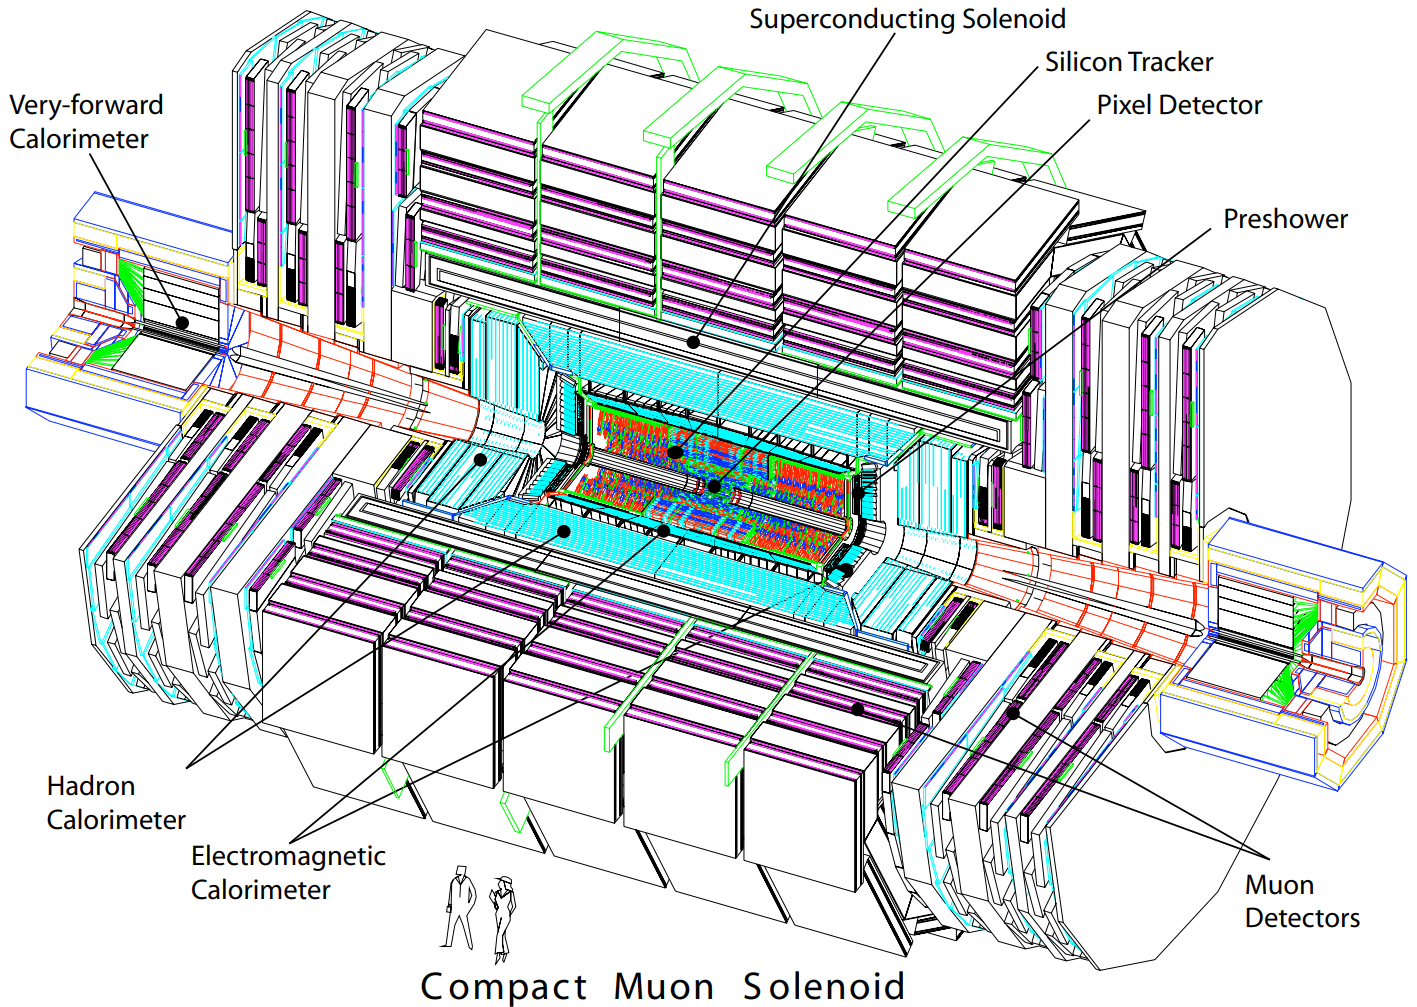
\includegraphics[width=0.9\textwidth]{Images/CMS.png}
	\captionof{figure}{Layout of the CMS experiment at the CERN LHC. (retrieved from~\parencite{CMS_2008}).}\label{fig_cms}
\end{center}

The detector is constructed from concentric layers of sub-detectors, as illustrated in Figure~\ref{fig_cms}. The innermost component is the silicon tracker, comprising a pixel detector and silicon strip tracker. It reconstructs the trajectories of charged particles and measures their transverse momenta ($p_T$) with a resolution of $\approx 0.7\%$ for 10~GeV particles within a pseudorapidity range of $|\eta| < 2.5$.



Surrounding the tracker is the calorimetric system. The electromagnetic calorimeter (ECAL) is made of lead-tungstate crystals. It is designed to measure electrons and photons with a high resolution of $\approx 0.6\%$ for 50~GeV electrons. The hadronic calorimeter (HCAL), located outside the ECAL, is a brass-scintillator sampling calorimeter that measures hadrons (e.g., charged pions, kaons, protons) with an energy resolution of $\approx 18\%$ for 50~GeV pions. Together, the ECAL and HCAL cover $|\eta| < 3$. The coverage is extended to $|\eta| < 5$ with steel and quartz-fiber hadron calorimeters in the forward regions.

A key feature of CMS is its large superconducting solenoid, which encloses the tracker and calorimeters. The solenoid is constructed from a niobium-titanium alloy and cooled to 4.2~K with liquid helium. It generates a uniform magnetic field of 3.8~T throughout the tracking volume, enabling precise momentum measurement from the curvature of charged particle tracks.

The outermost system is dedicated to muon identification and measurement. Gas-ionization detectors are embedded in the steel flux-return yoke that surrounds the solenoid. This system provides triggering and tracking capabilities for muons up to $|\eta| < 2.4$. The combination of the inner tracker and the muon system allows for a robust identification and momentum measurement of muons across a wide kinematic range.

The geometrical segmentation of the barrel and endcaps defines the detector's acceptance in terms of pseudorapidity. The central barrel provides optimal coverage for $|\eta| \lesssim 1.5$, while the endcaps extend the acceptance to $|\eta| \lesssim 2.5$ for the tracker and calorimeters, and to $|\eta| \lesssim 2.4$ for the muon system.

This segmentation impacts the detection efficiency. The silicon trackers are highly efficient in the barrel, where particles cross the layers perpendicularly. In the endcaps, the reduced hit multiplicity from shallow-angle traversals leads to a slight decrease in tracking efficiency and resolution. The calorimeters are also optimized to maintain performance across $\eta$, though the material budget and granularity vary.

Muon reconstruction performance exhibits regional differences. In the barrel, drift tubes (DTs) provide high spatial resolution, while in the endcaps, cathode strip chambers (CSCs) and resistive plate chambers (RPCs) are used to handle higher background rates and non-uniform magnetic fields. The assumed identification efficiency for muons (electrons) is 95\% (85\%), with a mis-identification rate of 0.3\% (0.6\%)~\parencite{CMS-PAS-FTR-13-014,CMS_MUON_17001,CMS_EGM_17001}.

For the identification of heavy-flavor jets, we adopt the DeepCSV algorithm~\parencite{CMS_BTV2016}. We use its ``medium'' working point, which provides a $b$-tagging efficiency of 70\% with a light-flavor jet misidentification rate of approximately 1\% across the entire $p_T$ spectrum. The ``loose'' (85\% efficiency, 10\% mis-id) and ``tight'' (45\% efficiency, 0.1\% mis-id) working points were also explored during the analysis optimization.

For hadronically decaying $\tau$ leptons ($\tau_h$), we use the DeepTau algorithm~\parencite{CMS_DeepTau}, which employs a deep neural network combining isolation and lifetime information to identify $\tau_h$ decay modes. The ``medium'' working point is chosen for this analysis, providing a $\tau_h$ identification efficiency of 70\% and a misidentification rate of 0.5\% for jets originating from light quarks and gluons. This working point was selected through an optimization process that maximized the discovery reach of the analysis.
